\section{Conclusion}

We present an online synthesis approach for runtime enforcers that guarantee local safety in multi-agent systems. The approach is decentralized and safe trajectories are synthesized onboard each agent as necessary. The algorithm we present does not require global information on the states of the other agents in the system. It only requires the information about the agents in the same communication group. With minor assumptions, we prove the correctness of the approach in enforcing safety and also prove that all the agents progress towards their original plan by bounding the maximum deviation and proving the absence of deadlocks. Finally, we show that if a $\ell$-stabilizing centralized shield can guarantee correctness, then $(\ell,|\Agents|^2 \ell)$--enforcers can also guarantee correctness.  We further prove that this synthesis scales efficiently with the number of agents. 

\begin{figure}[h]
    \centering
    \subfloat[Original trajectories]{
    \fbox{
    \begin{tikzpicture}
    \node[anchor=south west,inner sep=0] (image) at (0,0) {
    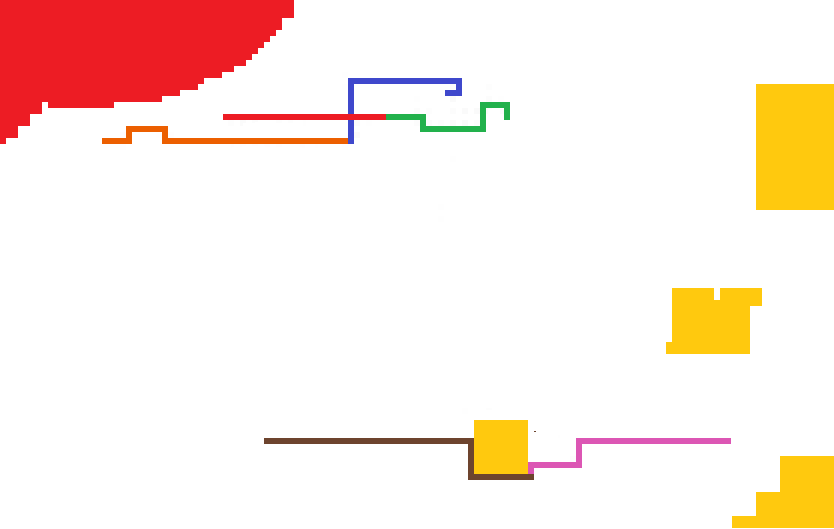
\includegraphics[width=.22\textwidth, height=40mm]{OnlineShield/orig.PNG}};
    \begin{scope}[x={(image.south east)},y={(image.north west)}]
    \begin{footnotesize}
    \node at (0.45,0.5) {collisions};
    \end{footnotesize}
    \draw[fill = black] (0.63,0.1) circle (1.3pt);
    \draw[fill = black] (0.42,0.73) circle (1.3pt);
    \draw[fill = black] (0.47,0.78) circle (1.3pt);
    \draw[<-,thick] (0.62,0.14) -- (0.49,0.44);
    \draw[<-,thick] (0.41,0.7)--(0.41,0.54);
    \draw[<-,thick] (0.48,0.75)--(0.48,0.54);
    \end{scope}
    \end{tikzpicture}
    }
    }
    \subfloat[Modified trajectories]{
    \fbox{
    \begin{tikzpicture}
     \node[anchor=south west,inner sep=0] (image) at (0,0) {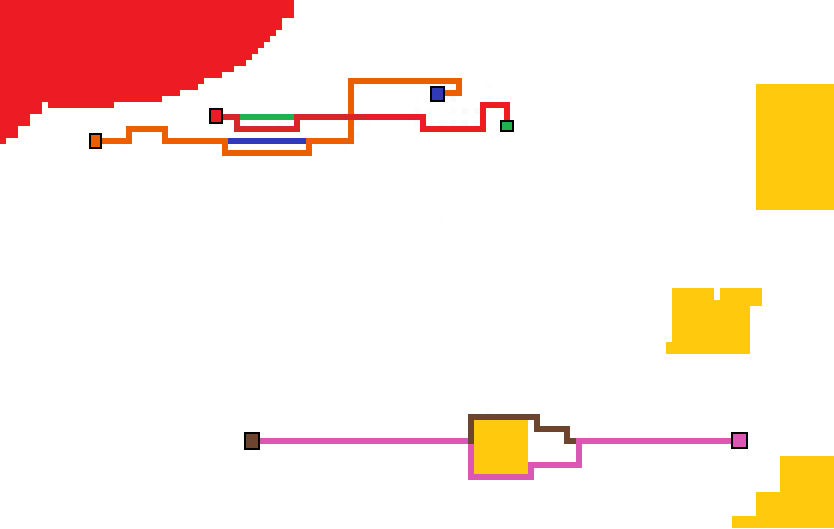
\includegraphics[width=.22\textwidth, height=40mm]{OnlineShield/mod.png}};
     \begin{scope}[x={(image.south east)},y={(image.north west)}]
     \draw[ultra thick, dotted] (0.32,0.75) circle (10.7pt);
     \draw[ultra thick, dotted] (0.62,0.17) circle (13pt);
     \begin{footnotesize}
     \node at (0.4,0.44) {deviations};
     \end{footnotesize}
     \draw[<-, thick] (0.35,0.62) -- (0.4,0.5);
     \draw[<-,thick] (0.54,0.27) -- (0.46,0.38);
     %\node at (0.19,0.55) {orange and};
     %\node at (0.17,0.45) {red agent};
     %\node at (0.17,0.35) {deviate};
     \end{scope}
   \end{tikzpicture}
   }
    %\fbox{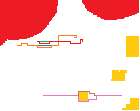
\includegraphics[width=.23\textwidth, height=40mm]{8agents_zoomed.png}}
    }
    
    \subfloat[Close-up of the deviation of the orange and red agents]{
    \fbox{
    \begin{tikzpicture}
     \node[anchor=south west,inner sep=0] (image) at (0,0) {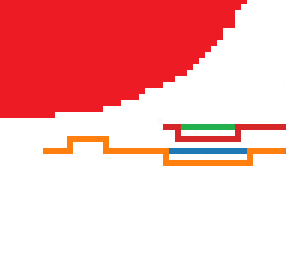
\includegraphics[width=0.21\textwidth,height=40mm] {OnlineShield/4agents_zoom.png}};
     \begin{scope}[x={(image.south east)},y={(image.north west)}]
     \begin{footnotesize}
     \node at (0.8,0.31) {orange agent deviates};
     \node at (0.82,0.57) {red agent deviates};
     %\node at (0.6,0.1) {min distance 2 is maintained};
     \end{footnotesize}
     \end{scope}
   \end{tikzpicture}
   }  
   }
   \caption{%The original trajectories of the orange, brown, and red agents are the same as the trajectories of the blue, pink, and green agents. However, they move in the opposite direction.  The modified trajectories ensure there is no collision between the agents. The deviation of the orange, red, and brown agents from their original trajectories illustrates the deviation caused by the corresponding enforcer.
    (a) The original trajectories of the orange, brown, and red agents are in conflict with the trajectories of the blue, pink, and green agents, respectively. The collisions are marked with black dots. (b) The initial positions of the agents are marked by squares. The modified trajectories ensure that there is no collision between the agents and that they are at least two units apart. The deviations are marked by the dashed black circles. (c) We show a close-up of the deviation of the orange and red agents from their original trajectories.
    %The black and the violet agents do not deviate since they do not collide with any other agent, showing minimal deviation.
    }
    \label{fig:8agents}
\end{figure}
